\documentclass[hide notes,intlimits]{beamer}

\mode<presentation>
{
  \usetheme[footline]{UAFshadealert}
  \setbeamercovered{transparent}
}

% frames are 128 millimeters by 96 millimeters

% load packages
\usepackage[english]{babel}
\usepackage[latin1]{inputenc}
\usepackage[T1]{fontenc}
\usepackage{amsmath,amssymb,wasysym}
\usepackage{lmodern}

\usepackage{tikz}
\usetikzlibrary{shapes,arrows,shadows}

\usepackage{empheq}
\usepackage{color}
\usepackage{animate}

\graphicspath{{figures/}}

% Some useful commands (from MPL)
\newcommand{\s}[1]{\ensuremath{\,\text{#1}}}
\newcommand{\unit}[1]{\ensuremath{\,\text{#1}}}

\definecolor{dark red}{HTML}{E41A1C}
\definecolor{dark green}{HTML}{4DAF4A}
\definecolor{dark violet}{HTML}{984EA3}
\definecolor{dark blue}{HTML}{084594}
\definecolor{dark orange}{HTML}{FF7F00}
\definecolor{light blue}{HTML}{377EB8}
\definecolor{light red}{HTML}{FB9A99}
\definecolor{light violet}{HTML}{CAB2D6}

\setbeamercolor{boxed}{fg=black,bg=uaf yellow}


\newenvironment{transbox}{%
  
\begin{tikzpicture}
    \node[drop shadow,rounded corners,text width=\textwidth,fill=white, fill opacity=0.6,text opacity=1] \bgroup
  }{
    \egroup;\end{tikzpicture}} 

\newenvironment{transbox-tight}{%
  \begin{tikzpicture}
    \node[drop shadow,rounded corners,fill=uaf yellow, fill opacity=0.75,text opacity=1] \bgroup
  }{
    \egroup;\end{tikzpicture}} 


% title page
\title[Better subglacial hydrology into PISM]{Better subglacial hydrology into \\ the Parallel Ice Sheet Model}
\subtitle{definitely a work in progress}

\author[Bueler \and van Pelt]{Ed Bueler\inst{*} and Ward van Pelt\inst{\dagger}}
\institute{\inst{*} University of Alaska Fairbanks \and %
           \inst{\dagger} IMAU, Utrecht, Netherlands}

\date{IGS June 2012}


\begin{document}

\setbeamertemplate{background canvas}
{
  % empty
}

% insert titlepage
\begin{frame}
  \titlepage
\end{frame}


\newcommand{\scream}[1]{\alert{\textbf{#1}}}

\begin{frame}
  \frametitle{PISM = Parallel Ice Sheet Model}

  \begin{center}
      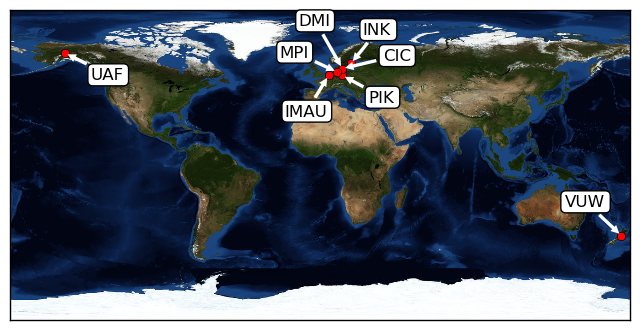
\includegraphics[width=80mm]{figs/pism-users-map}
  \end{center}

\vspace{-2mm}
  \begin{itemize}
  \item \alert{\large\texttt{www.pism-docs.org}}  and  \url{help@pism-docs.org}
  \item runs on laptops to supercomputers
  \item documented releases once a year
  \item \emph{User's Manual} with real modeling examples including Greenland Ice Sheet, Ross Ice Shelf, and St\"orglaciaren
  
  \bigskip
  \scriptsize
  \item[$\circ$] supported by the NASA Modeling, Analysis and Prediction (grant NNX09AJ38G)
  \item[$\circ$] jointly developed by UAF and the Potsdam Institute for Climate Impact Research
  \end{itemize}
\end{frame}


\newcommand{\whytitle}{why we need better subglacial hydrology}

\begin{frame}
  \frametitle{\whytitle}
  \framesubtitle{motivation 1}

\vspace{-6mm}
\begin{center}
  we are \scream{NOT} conserving mass (of liquid water)
\end{center}

\vspace{-5mm}
\begin{columns}
\begin{column}{0.5\textwidth}
  \begin{itemize}
    \item current basal hydrology in PISM has an independent ``can'' of porous till at each subglacial location %$\longrightarrow$
      \begin{itemize}
        \item[$\ast$] the can receives basal melt
        \item[$\ast$] ``overflows'' at 2m of water \dots overflow lost
        \item[$\ast$] \dots but it provides till yield stress in reasonable way
        \item[$\ast$] suitable for Siple coast ice streams (Tulaczyk et al 2000) %$\longrightarrow$
      \end{itemize}
    \item missing:
    
      \begin{center} \emph{lateral transport of water} \end{center}
  \end{itemize}
\end{column}
\begin{column}{0.5\textwidth}
\begin{center}
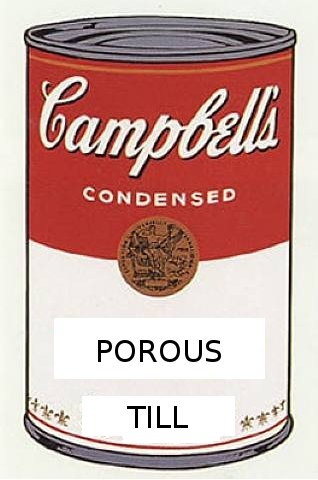
\includegraphics[height=0.3\textheight]{figs/till-warhol-soup}

%\vspace{1mm}

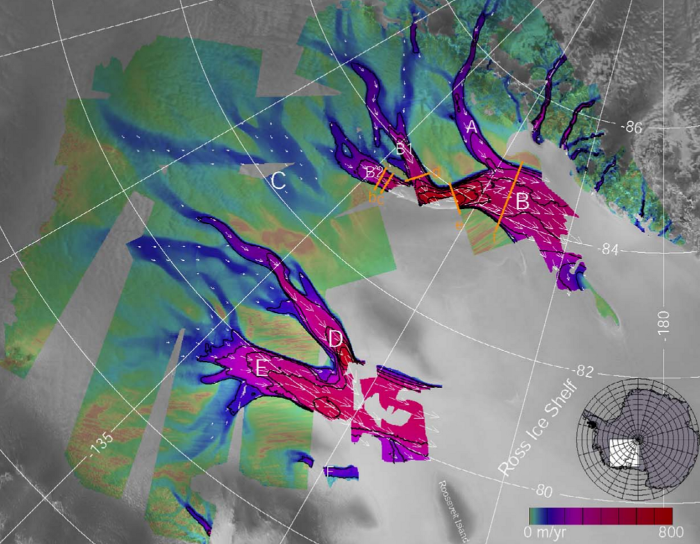
\includegraphics[height=0.45\textheight]{figs/siple}
\end{center}
\end{column}
\end{columns}
\end{frame}


\begin{frame}
  \frametitle{\whytitle}
  \framesubtitle{motivation 2}

\vspace{-6mm}
\begin{center}
  we \scream{ARE} conserving energy (better than before)
\end{center}
  
\vspace{-2mm}
  \begin{itemize}
    \item better energy conservation using enthalpy
    \item new basal melt rate equation
    %\item \emph{lots of water comes from dissipating gravitational potential energy, and some from geothermal energy}
  \end{itemize}

  \begin{center}
    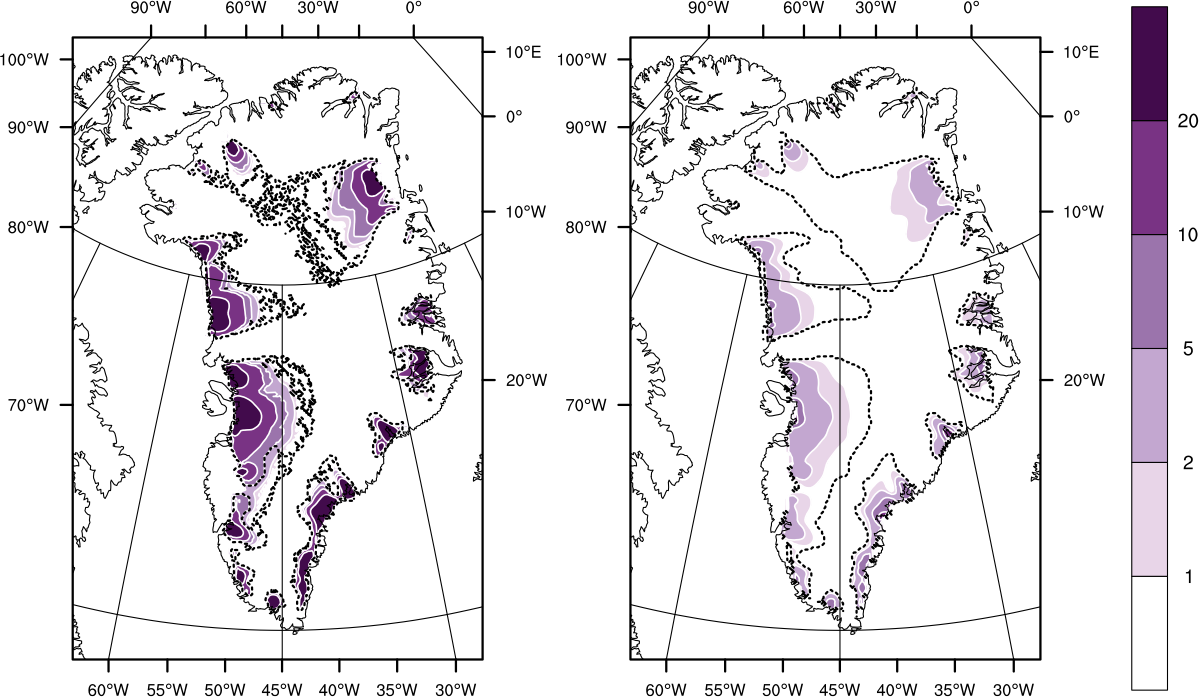
\includegraphics[height=0.6\textheight]{figs/enthalpy-model-crop}
    
    \medskip
    \scriptsize \textbf{left}: basal melt rate using \underline{enthalpy} \qquad \textbf{right}: basal melt rate using \underline{temperature}

    \tiny (from Aschwanden et al (2012) \emph{An enthalpy formulation for glaciers and ice sheets}, J. Glaciol.)
  \end{center}
\end{frame}


\begin{frame}
  \frametitle{example existing uses of PISM subglacial hydrology}

\begin{columns}
\begin{column}{0.5\textwidth}
\begin{center}
model the locations of all Antarctic ice streams without inversion

\vspace{13mm}

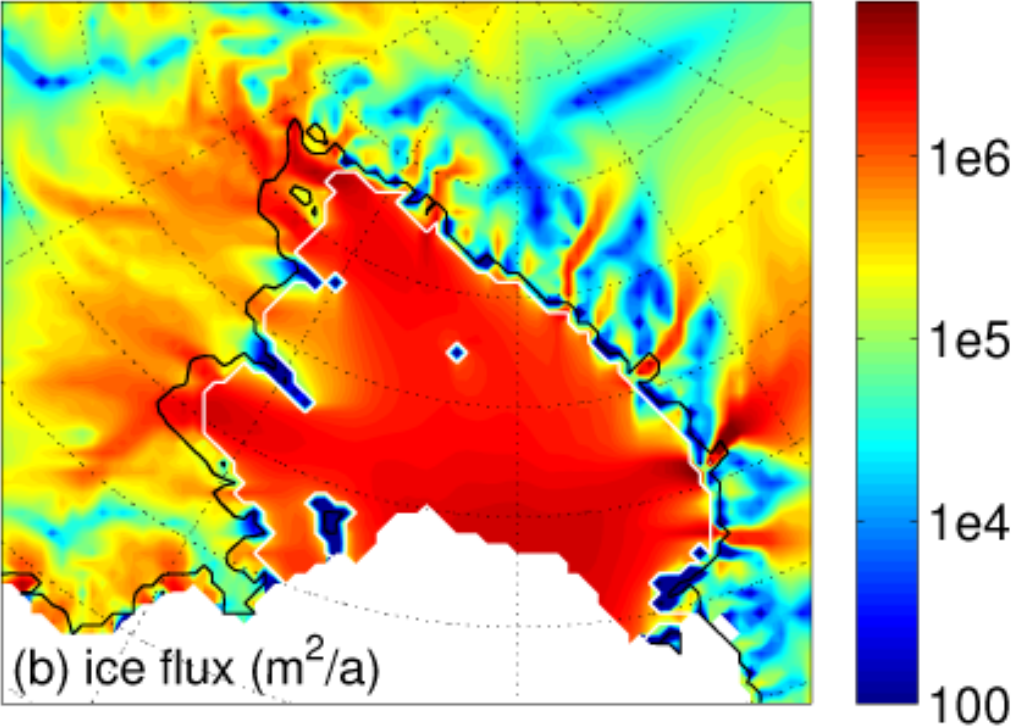
\includegraphics[width=0.9\textwidth]{figs/martin-fig12}

\vspace{8mm}

\medskip
\scriptsize (Martin et al., 2011, \emph{The Cryosphere})
\end{center}
\end{column}
\begin{column}{0.5\textwidth}
\begin{center}
study sliding/surging cyclicity in PISM

\bigskip
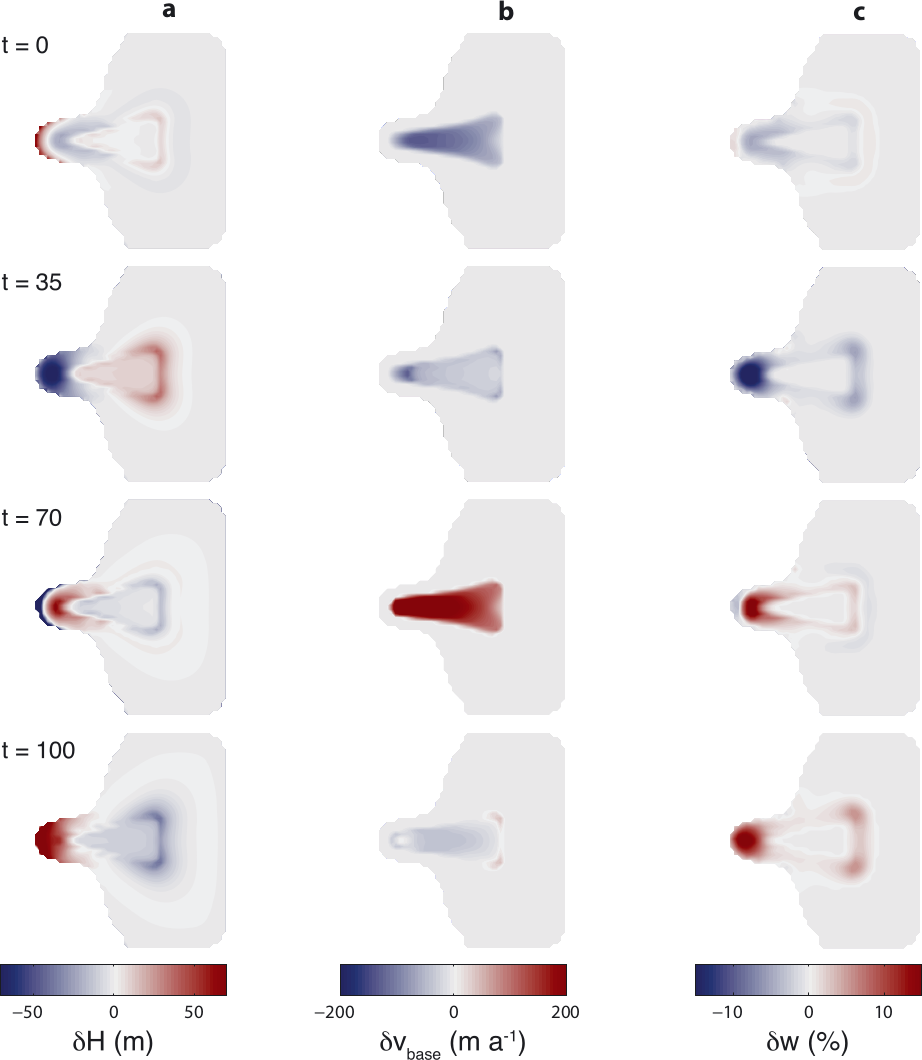
\includegraphics[width=0.8\textwidth]{figs/vanPeltOerlemans-fig4}

\medskip
\scriptsize (van Pelt \& Oerlemans, 2012, \emph{J.~Glaciol.})
\end{center}
\end{column}
\end{columns}
\end{frame}


\begin{frame}
  \frametitle{goal: improve PISM by adding mass-conserving subglacial hydrology}

subgoals:

\begin{enumerate}
  \item \scream{provide reasonable default behavior for new users}
  \item \scream{introduce a minimum number of new tunable parameters}
    %\item[$\ast$]<2-4> \dots that does no harm
  \item \scream{provide a playground for testing basal sliding models}
\end{enumerate}

\end{frame}




\begin{frame}
  \frametitle{elements of subglacial hydrology}
  \framesubtitle{we can agree on these?}

\newcommand{\bq}{\mathbf{q}}

  \begin{itemize}
    \item \textbf{conservation of mass}:
    
    $$W_t + \nabla \cdot \bq = m / \rho_w$$

where $W=$ spatially-averaged thickness of water layer, $\bq=$ flux, $m=$ supply rate ($\text{kg}\,\text{m}^{-2}\,\text{s}^{-1}$)

    \begin{onlyenv}<1>\item \textbf{hydraulic potential}:
    
    $$\phi = p_w + \rho_w g b$$

where $\phi=$ hydraulic potential, $b=$ bedrock elevation
    \end{onlyenv}

    \begin{onlyenv}<2>\item \textbf{hydraulic potential} {\color{blue} for top of water sheet}:
    
    $$\phi = p_w + \rho_w g (b{\color{blue} + W})$$

where $\phi=$ hydraulic potential, $b=$ bedrock elevation
    \end{onlyenv}

    \item \textbf{some kind of Darcy flow}:
    
    $$\bq = - \frac{K W}{\rho_w g} \nabla \phi$$
    
    where $K=$ hydraulic conductivity (\emph{not} constant in general)
    
    \medskip\medskip
    \scriptsize or \quad $\bq = - k W^\alpha |\nabla \phi|^{\beta - 2} \nabla \phi$ \quad etc.

  \end{itemize}

\end{frame}


\begin{frame}
  \frametitle{elements of subglacial hydrology}
  \framesubtitle{whence pressure?}

  \begin{itemize}
    \item combine previous three equations to get one equation in two unknown fields: $W$ and $p_w$
    \item an equation is needed to determine the pressure $p_w$
    \item some alternatives:
      \begin{itemize}
      \item[$\ast$] creep dominates, zero effective pressure (e.g.~slow subglacial lake):
        $$p_w = \rho_i g H$$
      \item[$\ast$] generates porous medium equation (Flowers \& Clarke 2002):
        $$p_w = \rho_i g H \left(\frac{W}{W_{\text{crit}}}\right)^\gamma$$
        where $\gamma=7/2$ and $W_{\text{crit}}=0.1$ m, for example
      \end{itemize}
  \end{itemize}

\end{frame}


\begin{frame}
  \frametitle{elements of subglacial hydrology}
  \framesubtitle{whence pressure? (more alternatives)}

  \begin{itemize}
    \item more possibilities:
      \begin{itemize}
      \item[$\ast$] physical models for opening and closure of a distributed system
        \begin{itemize}
        \item[$\circ$]  evolution equation for [$Y=$ average cavity depth] must be of the form
        $$Y_t = W_O - W_C$$
where $W_O$ is the total opening effect from a longish list of processes (wall melt, sliding, \dots) and $W_C$ is the total closing effect from a list of processes including creep (Hewitt, 2011)
        \item[$\circ$] indirectly this determines water pressure $p_w$
        \end{itemize}
      \item[$\ast$] but wait: there are channels, too! (R\"othlisberger 1972)

\begin{center}
\medskip
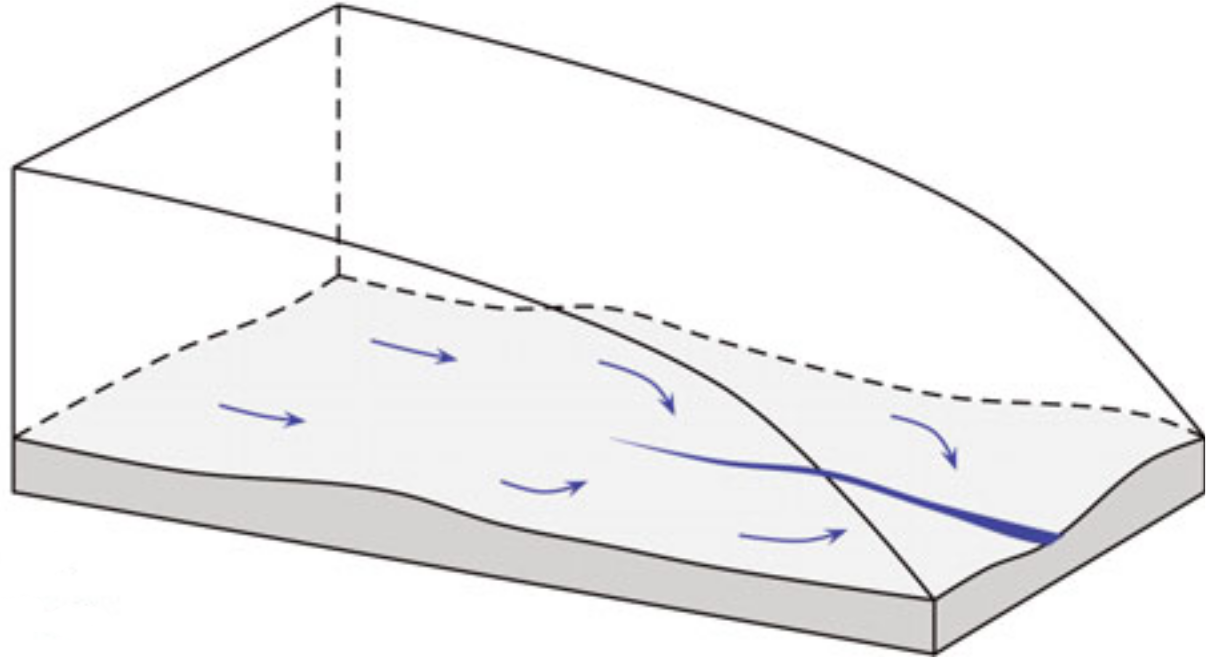
\includegraphics[width=0.4\textwidth]{figs/hewitt-cartoon} \tiny figure from (Hewitt, 2011)
\medskip
\end{center}
    \end{itemize}
  \end{itemize}
\end{frame}


\begin{frame}
  \frametitle{elements of subglacial hydrology}
  \framesubtitle{whence pressure? (yet more alternatives \dots from Vancouver, B.C.~area as usual)}

\begin{columns}
\begin{column}{0.6\textwidth}
  \begin{itemize}
  \item and more possibilities:
  \begin{itemize}
  \item[$\ast$]  Creyts \& Schoof (2009): bed protrusions stabilize sheet flow (c.f.~Walder 1982)

  \bigskip
  \item[$\ast$]  Schoof (2010): fixed-location 2D network of channels (top figure)
      \begin{itemize}
      \item[$\circ$] grid-refinement limit not known?
      \end{itemize}
      
  \bigskip
  \item[$\ast$]  Hewitt and Schoof and Werder (2012)
      \begin{itemize}
      \vspace{-3mm}
      \item[$\circ$] elliptic variational inequality determines water pressure from bounds
      $$0 \le p_w \le \rho_i g H$$
      \item[$\circ$] may be large areas where $p_w = \rho_i g H$ anyway
      \end{itemize}
  \end{itemize}
  \end{itemize}
\end{column}

\begin{column}{0.4\textwidth}
\begin{center}
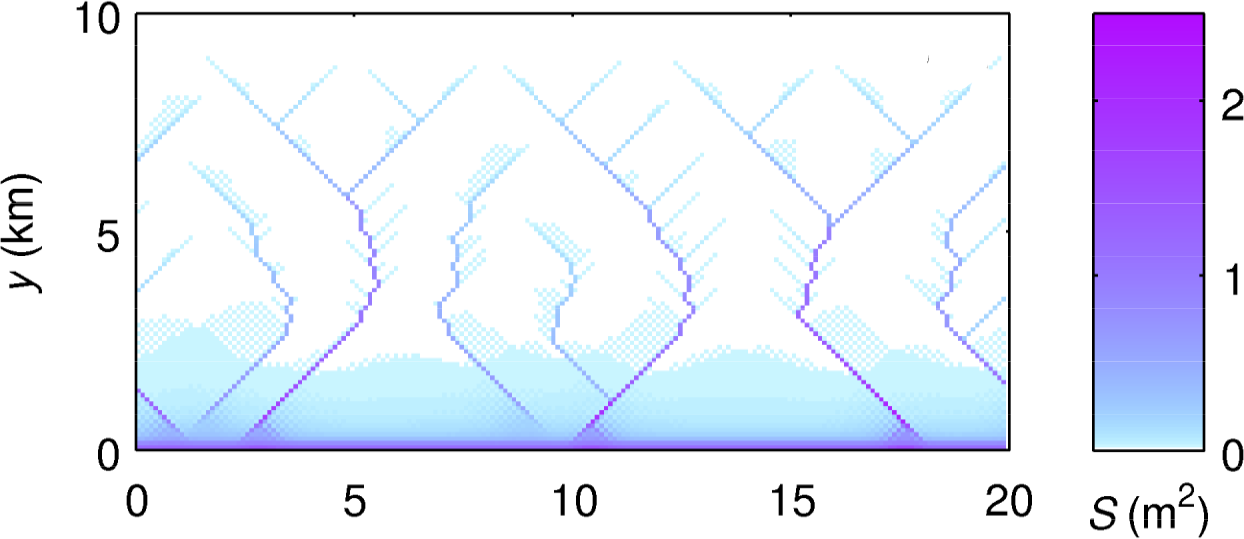
\includegraphics[width=1.0\textwidth]{figs/schoof-channels}

\vspace{20mm}

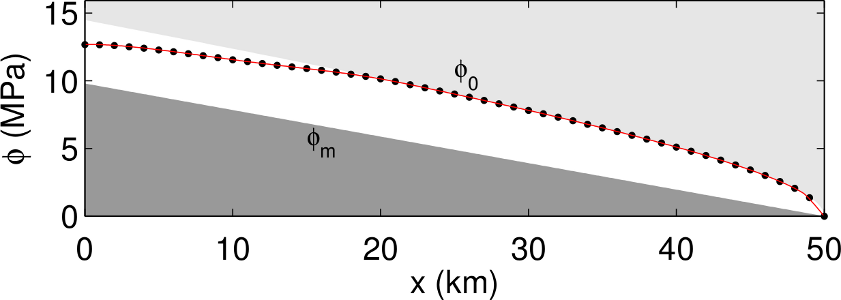
\includegraphics[width=1.0\textwidth]{figs/schoof-overburden}
\end{center}
\end{column}
\end{columns}

\end{frame}


\begin{frame}
  \frametitle{TMI}

  \begin{itemize}
  \item too much information!
  \item \dots and too many tunable parameters
    \begin{itemize}
    \item[$\ast$] even though I \emph{like} elliptic variational inequalities
    \end{itemize}
  \item yes, we hope to explore these possibilities in PISM
  \item but it has finally dawned on us:
  
  \begin{center}
  \emph{exploring processes through modeling is different from improving default behavior for ice sheet simulation}
  \end{center}
  \end{itemize}
\end{frame}


\begin{frame}
  \frametitle{back to something basic}

  \begin{itemize}
    \item recall the simple model where creep dominates:
    		$$p_w = \rho_i g H$$
    \item then hydraulic potential comes from three heights:
    \begin{align*}
      \phi &= \rho_i g H + \rho_w g (b+W) \\
           &= \rho_i g \,h + (\rho_w - \rho_i) g \,b + \rho_w g \,W
    \end{align*}
    \emph{note relative sizes of coefficients}
    \item<2-3> combining all equations gives:
       $$\boxed{W_t + \nabla\cdot\left(\mathbf{v} W\right) = \nabla \cdot(K W \nabla W) + m / \rho_w}$$
      \begin{itemize}
      \vspace{-3mm}
      \item[$\ast$] where $\mathbf{v} = - K \left[r \nabla h + (1-r) \nabla b\right]$  \qquad (and $r = \rho_i/\rho_w$)
      \item[$\ast$] a nonlinear advection-diffusion equation
      \end{itemize}
    \item<3> \scriptsize generalization with one more tunable parameter $0<s<1$: \quad $p_w = s\, \rho_i g H$
  \end{itemize}
\end{frame}


\begin{frame}
  \frametitle{velocity and time scales in the ``basic'' model}

  \begin{itemize}
    \item again, if $r = \rho_i/\rho_w$ then
      $$\mathbf{v} = - K \left[r \nabla h + (1-r) \nabla b\right]$$
    \item what happens with real data (\emph{ALBMAPv1}) for $h(x,y)$ and $b(x,y)$?
    \begin{center}
    \medskip
     \qquad 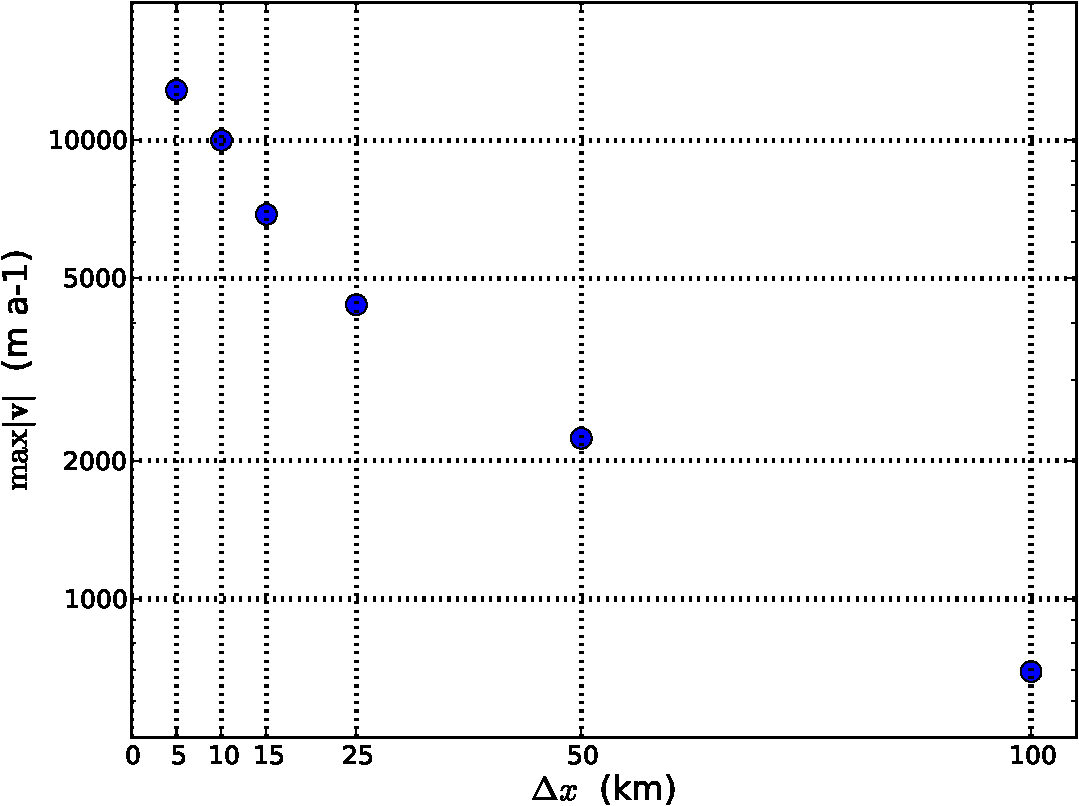
\includegraphics[width=0.4\textwidth]{figs/vresults}
    \medskip
    \end{center}
       \small
       \begin{itemize}
       \item[$\ast$] so we probably need a regularization (smoothing or cap) on $\mathbf{v}$
       \end{itemize}
       \normalsize
    \item diffusivity $D = K W \sim 10^{-3} \, (\text{m}^2 \text{a}^{-1})$ if $K=10^{-3} \,\text{m}\,\text{a}^{-1}$ and $W=1$ m, which is tiny \small \dots but big $K$ gives a regularization
  \end{itemize}

\end{frame}


\begin{frame}
  \frametitle{Antarctic Ice Sheet example: where does the water concentrate?}

  \begin{itemize}
    \item models like this have been used to suggest distribution of subglacial lakes in Antarctica
    \item here some toy results with $m/\rho_w = 1 \,\,\text{cm}\,\text{a}^{-1}$ uniformly over whole ice sheet
    \item FIXME: show for EAIS
  \end{itemize}

\end{frame}


\begin{frame}
  \frametitle{practical PISM benefit with basic model}
 
\begin{itemize}
\item  \scream{report the amount of subglacial water delivered at each outlet}
\item \dots like we can report the amount of ice delivered at each outlet
\item \dots through automatic identification of ``drainage basins''
  \begin{itemize}
  \item[$\ast$] e.g.~Jakobshavn basins below
  \end{itemize}
\end{itemize}

\vspace{-5mm}

\begin{columns}
\begin{column}{0.5\textwidth}
\begin{center}
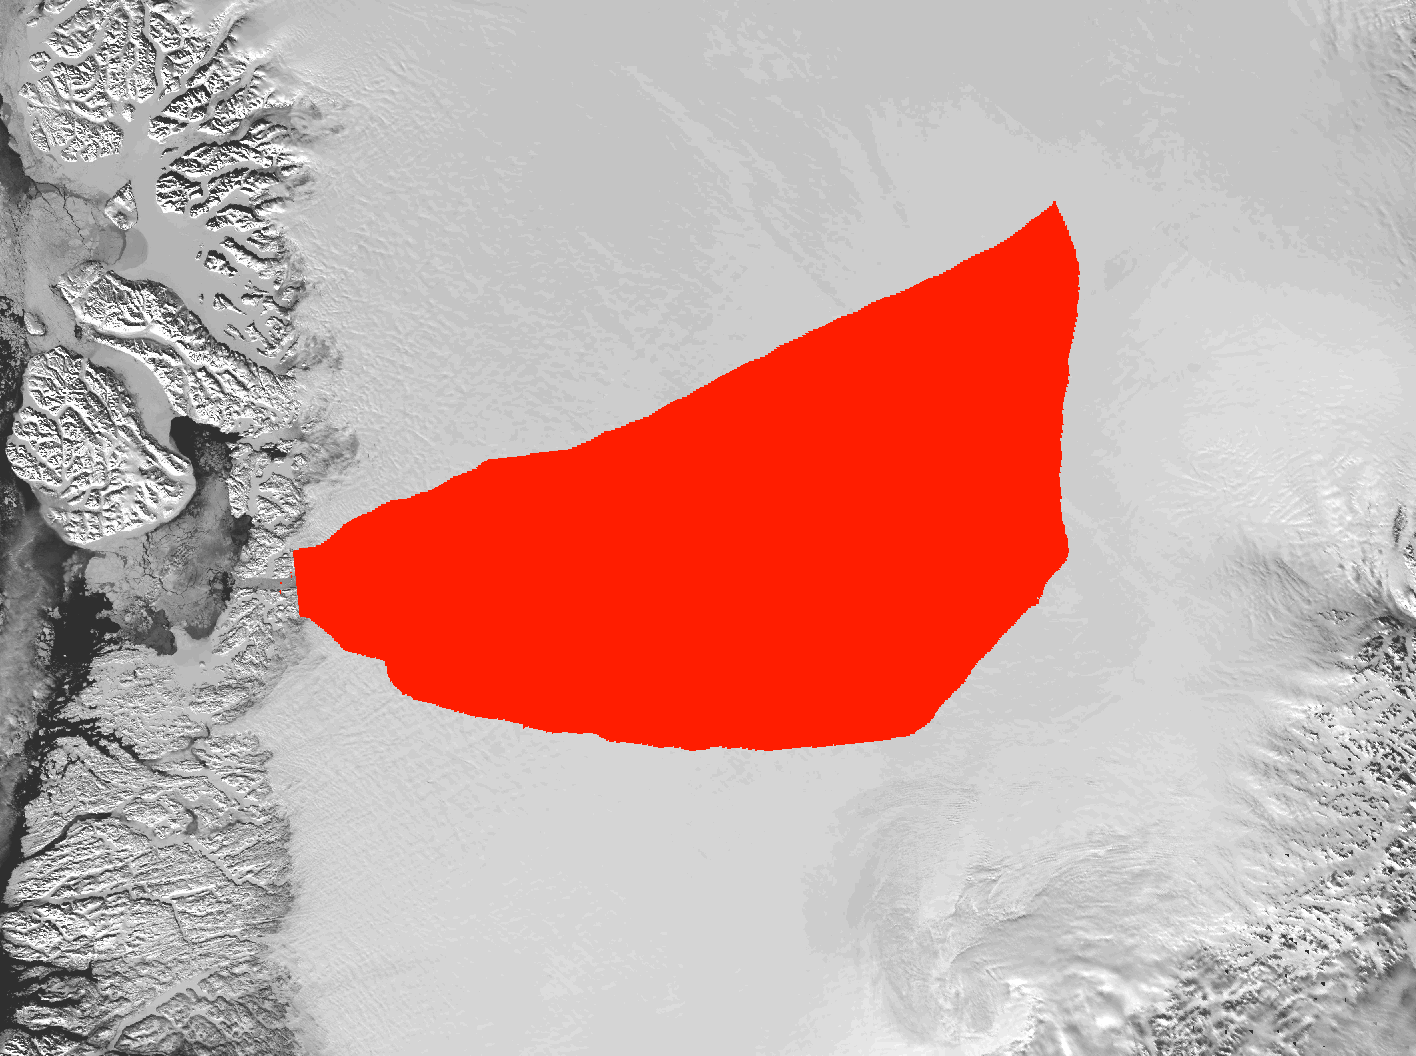
\includegraphics[width=0.85\textwidth]{figs/ftt-mask}

basin for $-\nabla h$ flow,

\phantom{where $\phi$}

for ice
\end{center}
\end{column}
\begin{column}{0.5\textwidth}
\begin{center}
\vspace{0.5mm}

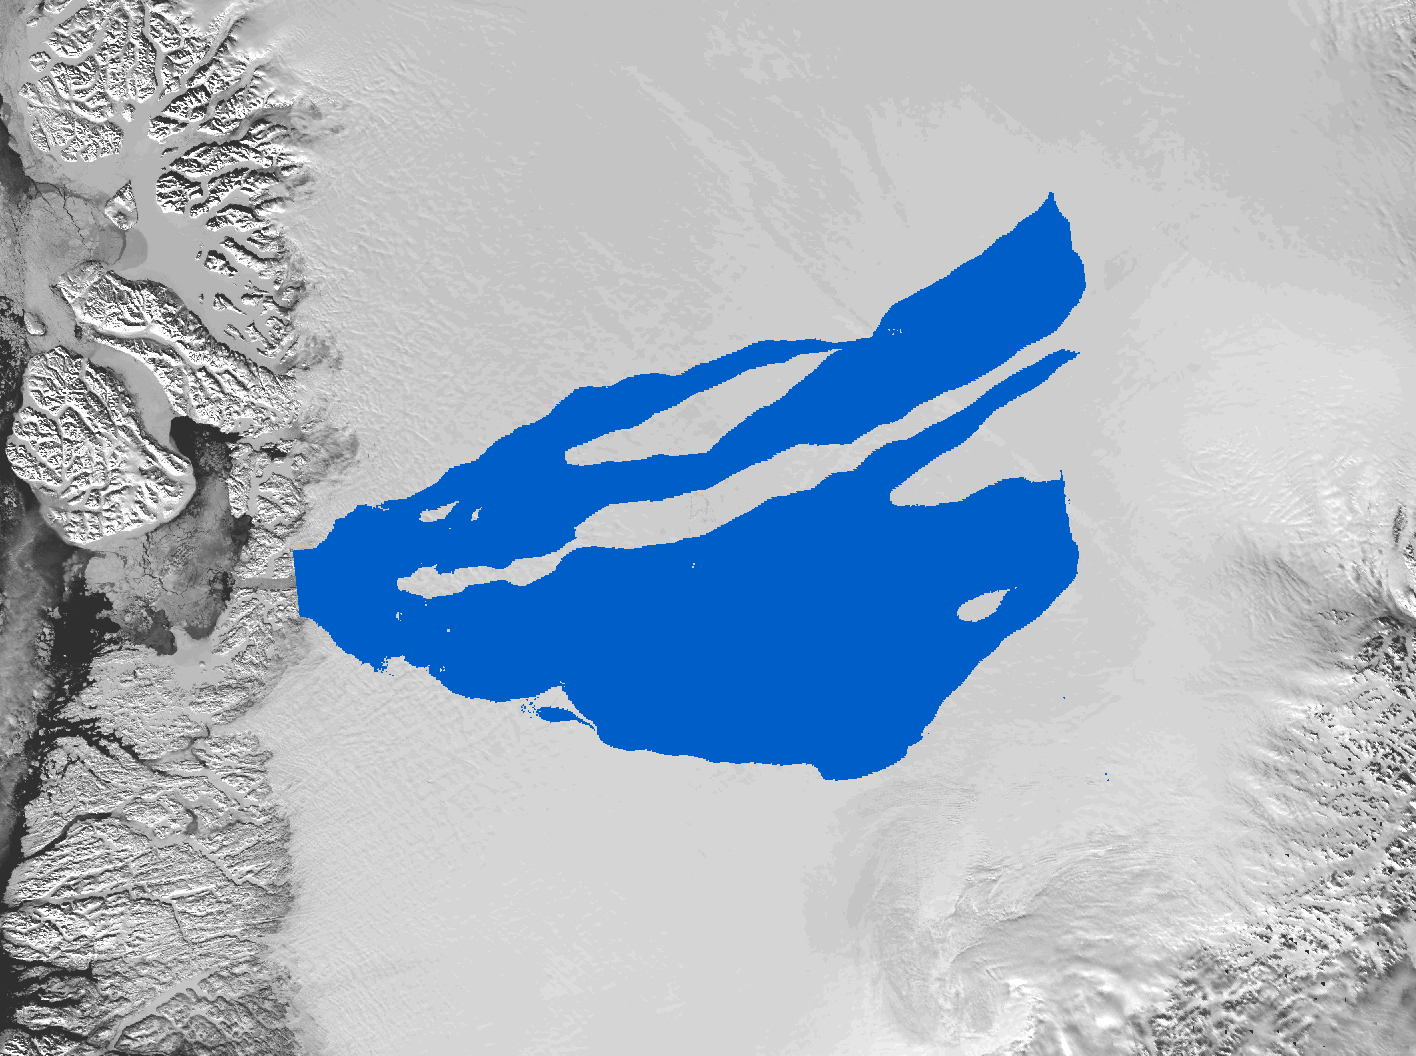
\includegraphics[width=0.85\textwidth]{figs/hydro-mask}

basin for $-\nabla \phi$ flow,

where $\phi = \rho_i g H + \rho_w g b$,

for subglacial water
\end{center}
\end{column}
\end{columns}

\end{frame}


\setbeamertemplate{background canvas}
{
  \tikz{\node[inner sep=0pt,opacity=0.3] {\includegraphics[width=\paperwidth]{figs/crop-andy-66}};}
} 


\begin{frame}
  \frametitle{summary}

  \begin{itemize}
  \item we plan to put this ``basic'' model in PISM
  \item then extend it to enable modelling of more dynamic subglacial drainage systems
    \begin{itemize}
    \small
    \item[$\ast$] nontrivial aspect which everyone knows: water flux and wall melt term in the opening/closing equation  leads to concentrated water flow in channels
    \item[$\ast$] the spatial average of that process must be captured
    \end{itemize}
    \normalsize
  \item we are aware of the danger of building a model whose parameters cannot be identified
    \begin{itemize}
    \small
    \item[$\ast$] too much depends on surface observations of flow
    \end{itemize}
    \normalsize
  \end{itemize}

\vspace{17mm}
  \begin{center}
  \tiny \emph{Thanks for help with figures: Andy Aschwanden, Sarah Child, Brad Gooch}
  \end{center}
\end{frame}








\end{document}
